% This is the Reed College LaTeX thesis template. Most of the work
% for the document class was done by Sam Noble (SN), as well as this
% template. Later comments etc. by Ben Salzberg (BTS). Additional
% restructuring and APA support by Jess Youngberg (JY).
% Your comments and suggestions are more than welcome; please email
% them to cus@reed.edu
%
% See http://web.reed.edu/cis/help/latex.html for help. There are a
% great bunch of help pages there, with notes on
% getting started, bibtex, etc. Go there and read it if you're not
% already familiar with LaTeX.
%
% Any line that starts with a percent symbol is a comment.
% They won't show up in the document, and are useful for notes
% to yourself and explaining commands.
% Commenting also removes a line from the document;
% very handy for troubleshooting problems. -BTS

% As far as I know, this follows the requirements laid out in
% the 2002-2003 Senior Handbook. Ask a librarian to check the
% document before binding. -SN

%%
%% Preamble
%%
% \documentclass{<something>} must begin each LaTeX document
\documentclass[12pt,twoside]{reedthesis}
% Packages are extensions to the basic LaTeX functions. Whatever you
% want to typeset, there is probably a package out there for it.
% Chemistry (chemtex), screenplays, you name it.
% Check out CTAN to see: http://www.ctan.org/
%%
\usepackage{graphicx,latexsym}
\usepackage{amssymb,amsthm,amsmath}
\usepackage{longtable,booktabs,setspace}
\usepackage{chemarr} %% Useful for one reaction arrow, useless if you're not a chem major
\usepackage[hyphens]{url}
\usepackage{rotating}
\usepackage{natbib}
\usepackage{pgfplots}
\pgfplotsset{compat=1.5}
\usepackage[alsoload=astro]{siunitx}
% Comment out the natbib line above and uncomment the following two lines to use the new
% biblatex-chicago style, for Chicago A. Also make some changes at the end where the
% bibliography is included.
%\usepackage{biblatex-chicago}
%\bibliography{thesis}

\usepackage{fbb} % other fonts are available like times, bookman, charter, palatino

\title{N-Body Simulations of Barred Galaxies}
\author{Thomas B Malthouse}
% The month and year that you submit your FINAL draft TO THE LIBRARY (May or December)
\date{Summer 2017}
\division{Mathematics and Natural Sciences}
\advisor{J Powell}
%If you have two advisors for some reason, you can use the following
%\altadvisor{Your Other Advisor}
%%% Remember to use the correct department!
\department{Physics}


\setlength{\parskip}{1.5em}

\DeclareSIUnit[]\solar
{\mathrm{\ensuremath{M}}_\odot}
\DeclareSIUnit[]\year
{\mathrm{\ensuremath{yr}}}


%%
%% End Preamble
%%
%% The fun begins:
\begin{document}

  \maketitle
  \frontmatter % this stuff will be roman-numbered
  \pagestyle{empty} % this removes page numbers from the frontmatter

% Acknowledgements (Acceptable American spelling) are optional
% So are Acknowledgments (proper English spelling)
    \chapter*{Acknowledgements}
	I want to thank a few people.

% The preface is optional
% To remove it, comment it out or delete it.
    \chapter*{Preface}
	This is an example of a thesis setup to use the reed thesis document class.



    \chapter*{List of Abbreviations}
		You can always change the way your abbreviations are formatted. Play around with it yourself, use tables, or come to CUS if you'd like to change the way it looks. You can also completely remove this chapter if you have no need for a list of abbreviations. Here is an example of what this could look like:

	\begin{table}[h]
	\centering % You could remove this to move table to the left
	\begin{tabular}{ll}
		\textbf{ABC}  	&  American Broadcasting Company \\
		\textbf{CBS}  	&  Columbia Broadcasting System\\
		\textbf{CDC}  	&  Center for Disease Control \\
		\textbf{CIA}  	&  Central Intelligence Agency\\
		\textbf{CLBR} 	&  Center for Life Beyond Reed\\
		\textbf{CUS}  	&  Computer User Services\\
		\textbf{FBI}  	&  Federal Bureau of Investigation\\
		\textbf{NBC}  	&  National Broadcasting Corporation\\
	\end{tabular}
	\end{table}


    \tableofcontents
% if you want a list of tables, optional
    \listoftables
% if you want a list of figures, also optional
    \listoffigures

% The abstract is not required if you're writing a creative thesis (but aren't they all?)
% If your abstract is longer than a page, there may be a formatting issue.
    \chapter*{Abstract}
	The preface pretty much says it all.

	\chapter*{Dedication}
	You can have a dedication here if you wish.

  \mainmatter % here the regular arabic numbering starts
  \pagestyle{fancyplain} % turns page numbering back on

%The \introduction command is provided as a convenience.
%if you want special chapter formatting, you'll probably want to avoid using it altogether

    \chapter*{Introduction}
         \addcontentsline{toc}{chapter}{Introduction}
	\chaptermark{Introduction}
	\markboth{Introduction}{Introduction}
	% The three lines above are to make sure that the headers are right, that the intro gets included in the table of contents, and that it doesn't get numbered 1 so that chapter one is 1.

% Double spacing: if you want to double space, or one and a half
% space, uncomment one of the following lines. You can go back to
% single spacing with the \singlespacing command.
% \onehalfspacing
% \doublespacing

The Milky Way is an entirely unextraordinary galaxy. Its hallmark spiral arms---visible in the night sky, stretching from horizon to horizon---are shared by about 60\% of galaxies in our universe \citep{apm-bgc}. A bar---a large collection of stars passing through the galactic center, prominent in renderings of the Milky Way---is also found around two in three other spiral galaxies---meaning about 40\% of known galaxies are of the same classification as ours. These extensive similarities mean that studying the evolution and structure of the Milky Way can provide insights about galactic behavior in general, and that observing other galaxies can reveal the past and future of out own.

\section*{Disks}
The Milky Way has two main disks which hold the vast majority of visible matter in the galaxy and give rise to its spiral structure. The \emph{thin disk} is the more visible of the two, composed mainly of main-sequence stars and clouds of gas and dust \citep{galaxies-in-universe}. Its vertical density scale height---the distance over which its density decreases by a factor of $e$---is about $\SI{350}{\parsec}$---very thin compared to its radius of about $\SI{25}{\kilo\parsec}$. This thinness comes from its young age, since the stars that compose it are less likely to have had their orbits perturbed---especially in the chaotic period about $\SI{9}{\giga\year}$ ago. The thin disk accounts for about 97\% of the galaxy's (normal) mass and holds nearly all galactic dynamism and stellar formation.

The other disk, referred to as the \emph{dark disk} or \emph{thick disk}, is far older and less dynamic \citep{starrfield-thick-disk}. Composed of stars formed $\SI{10}{\giga\year}$ to $\SI{12}{\giga\year}$ ago, it is very faint and hard to detect---all the bright stars burned out long ago, and the only ones left are low-magnitude red dwarfs and K-class stars. These stars' orbits also tend to be less regular, since they've had time to be perturbed and pushed into new orbits, especially during the chaotic initial organization of the Milky Way $\SI{10}{\giga\year}$ ago---resulting in a scale height of about $\SI{1}{\kilo\parsec}$. Because its stars are so steady-burning and the complete lack of gas and dust, the thick disk is very stable and exhibits none of the dynamism seen in the thin disk. It accounts for only about 3\% of the regular matter in the galaxy, with a total mass of about $\SI{1e10}{\solar}$.
Note that the name \emph{dark disk} refers to the low luminosity of the stars within, and has no relation to the dark matter discussed below.

\section*{Metallicity and Age}
The easiest way to determine which disk a star is in is to look at its metallicity (the amount of metal in the star.) This can be measured by looking at the strength of various emission spectra, since elements like iron have very distinct emission lines. These heavy elements are only formed when large stars reach the end of their life, and so their concentration has steadily increased over time as more large stars form and die. Old stars dating back to the formation of the galaxy (like those of the thick disk) tend to have very ``clean'' emission spectra, with very little other than hydrogen and helium, while younger stars have strong magnesium and iron lines.

Metallicity isn't a perfect way to measure the age of a star. Metal concentrations vary widely across both space and time, and two stars forming at the same time may have very different metallicities. However, when looking at a large and statistically representative sample of stars, a high metallicity indicates a younger age \citep[pp. 885]{modern-astrophysics}.

\section*{The Stellar Halo}

The disks extend to about $\SI{25}{\kilo\parsec}$ from the galactic center, and contain practically all the mass within that radius. Past that point, however, stars are distributed far more chaotically. The thin plane disappears, and stellar orbits become more spherically distributed. The composition of individual stars in the halo is similar to those in the thick disk---old, dim, and unchanging. However, the halo is also home to many globular clusters, groups of tens or hundreds of thousands of stars that act like small galaxies in their own right. These clusters continue to create new stars, and most of the light coming from the halo is from globular clusters.

Measurements of stellar velocities have long predicted that the mass of the halo dominates the mass of the galaxy---about 95\% of galactic mass must be in the halo for the observed velocity curves to hold. Since the halo was known not to be made up of gas and dust (otherwise its extinctive properties would be easy to measure), astronomers long though that the halo contained vast numbers of dense, dark bodies, such as lone planets, dim stars, black holes, and neutron stars---referred to as MACHOs, or Massive Astrophysical Compact Halo Object. Gravitational lensing observations disproved this theory, however, when they capped the mass percentage of MACHOs at about 15\% of the mass of the galaxy. The remainder of the mass was some strange material, spherically distributed throughout the universe, that interacts with nothing but gravity.

\section*{Dark Matter}
As that strange material was further studied (as much as it is possible to study something so elusive), more of its properties were discovered. This \emph{dark matter} seems to be made up of WIMPS (Weakly Interacting Massive Particles), which only interact via gravity and the weak force. Being collisionless (since it does not interact with the electromagnetic force), it does not coalesce and form clouds and stars like regular matter, which is how it has maintained its spherical distribution for so long.

This dark matter has a density of
\begin{equation}
    \rho(r) = \frac{\rho_0}{\left(\frac{r}{a}\right)\left(1+\frac{r}{a}\right)^2}
\end{equation}
where $\rho_0$ is the maximum density and $a$ is proportional to the size of the galaxy. This function is referred to as the NFW profile (named after its creators, Navarro, Frank, and White), and is highly accurate for all observed spiral galaxies. For the Milky Way, the simplified equation
\begin{equation}
    \rho(r) = \frac{\rho_0}{1+\left(\frac{r}{1}\right)^2}
\end{equation}
also returns satisfactory results. However, both these equations appear to suffer from a major problem. If we use them to calculate the total mass of the dark matter in a galaxy, integrating from 0 to $\infty$, it appears that a galaxy has an infinite mass, as follows:
\begin{equation}
    \int\limits_{0}^{\infty} \rho(r) 4 \pi r^2 \, \text{d}r = \infty
\end{equation}
Since we know this is not true, there must be a cutoff point where the law no longer holds. As it turns out, in local groups like our own, the dark matter halos are so large that they border one another---providing a natural cutoff point and a solution to our problem \citep[pp. 196]{galaxies-in-universe}.

\section*{Coordinate Systems}

To identify and keep track of objects in the sky, we need to create a coordinate system. A number of natural possibilities spring to mind. The three most useful are detailed below.

\subsection*{Equatorial Coordinates}

An equatorial coordinate has two components---a \emph{right ascension}, and a \emph{declination}. To find this coordinate, find the location on the Earth's surface where the object of interest is directly overhead, in the very middle of the sky. The right ascension is the angle between the nearest point on the equator and the vernal equinox (which is defined to be the point where the equator crosses the ecliptic). The declination is then the angle between the current point and that nearest equatorial point. This coordinate system is very ancient, dating back millennia. Figure \ref{equatorial-coords} shows the process of finding such a coordinate.

\begin{figure}[p]
    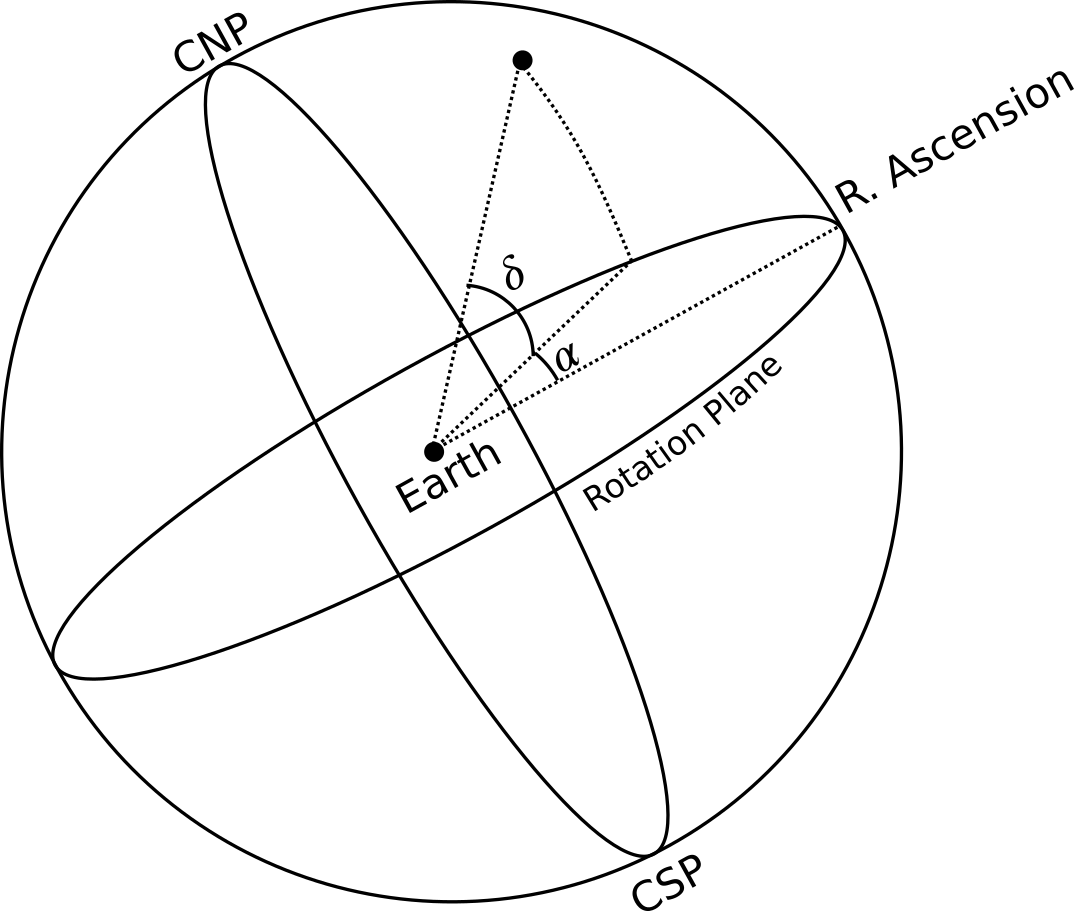
\includegraphics{imgs/equat.png}
    \caption{This figure shows the process of finding an equatorial coordinate. CNP and CSP refer to the celestial north and south poles, respectively. R. Ascension refers to the right ascending node, where the Earth's rotational plane crosses its orbital plane.}
    \label{equatorial-coords}
\end{figure}

\subsection*{Galactic Coordinates}

This coordinate system is similar to the equatorial system, but the declination is measured from the galactic plane instead of the equatorial plane. The right ascension is then defined to be the angle between the projection of the body of interest on the galactic plane and the vector between the Sun and galactic center. Figure \ref{galactic-coords} shows this process in more detail. Although harder to calculate from the surface of the earth, this system is more natural when studying bodies traveling close to the Sun. The standard notation and conversions between the two systems are given below:

\begin{tabular}{lll} \toprule
    Measurement & Equatorial Notation & Galactic Notation \\ \midrule
    Right Ascension &  $\delta$       & $b$               \\
    Declination     &  $\alpha$       & $\ell$            \\ \bottomrule
\end{tabular}

\begin{equation}
    \sin b = \sin \delta_{NGP} \sin \delta + \cos \delta_{NGP} \cos \delta \cos (\alpha-\alpha_{NGP})
\end{equation}
\begin{equation}
    \sin \delta = \sin \delta_{NGP} \sin b + \cos \delta_{NGP} \cos b \cos{\ell_{NCP} - \ell}
\end{equation}
Where $\delta_{NGP} = \ang{27;7;41.7}$ and $\ell_{NCP}=\ang{123;55;55.2}$, as determined by the tilt of the earth and its orientation relative to the galactic plane. These equations can also be inverted to find $\ell$ and $\alpha$ \citep[pp. 900]{modern-astrophysics}.

\begin{figure}[p]
    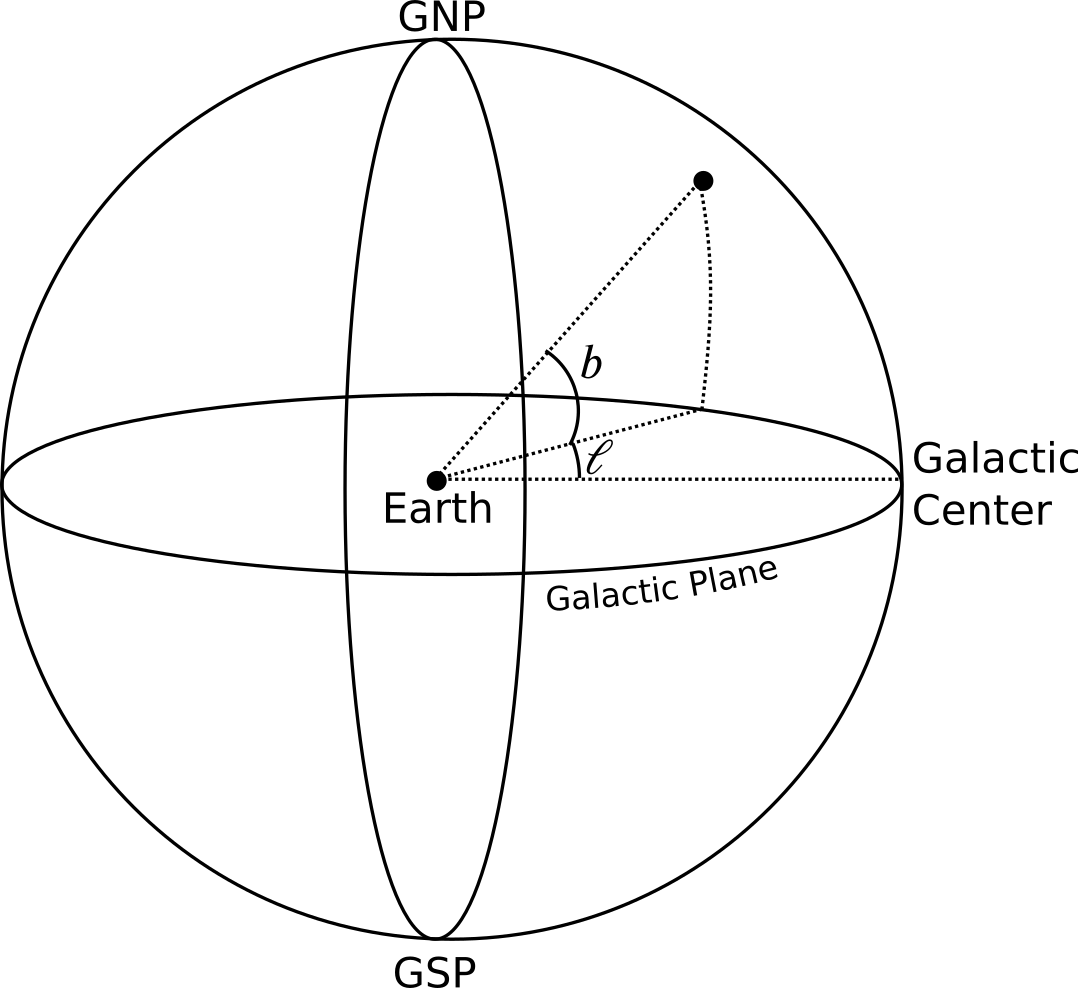
\includegraphics{imgs/galactic}
    \caption{This figure shows the process of finding a galactic coordinate. GNP and GSP refer to the galactic north and south poles, respectively.}
    \label{galactic-coords}
\end{figure}

\subsection*{Cylindrical Coordinates}

The two coordinate systems discussed earlier are well-suited for positional observations from the Earth at a given point in time, but perform poorly over long timeframes. As the sun travels around its orbit, the coordinates of an object change even if it has not moved at all---not an ideal behavior from a reference system. The cylindrical coordinate system, with a reference point at the center of the universe solves these concerns. Unlike the others, it is a three-component coordinate system: $R$ is the radial distance along the plane, increasing outwards; $\theta$ is the angular position, and increases in the direction of rotation; and $z$ is the height above (or below) the plane, increasing towards the north, as shown in figure \ref{cylindrical-coords}. These coordinates also produce a natural (and commonly used) velocity coordinate system, as described below \citep{modern-astrophysics}:
\begin{equation}
    \Pi \equiv \frac{dR}{dt} \hspace{2cm} \Theta \equiv R\frac{d\theta}{dt} \hspace{2cm} Z \equiv \frac{dz}{dt}
\end{equation}

Note that, because the galaxy rotates clockwise when viewed from the north pole, this is a left-handed coordinate system rather than a more-standard right-hand system. Fortunately, we do not need to take any cross-products, so this does not cause any problems.

\begin{figure}[p]
    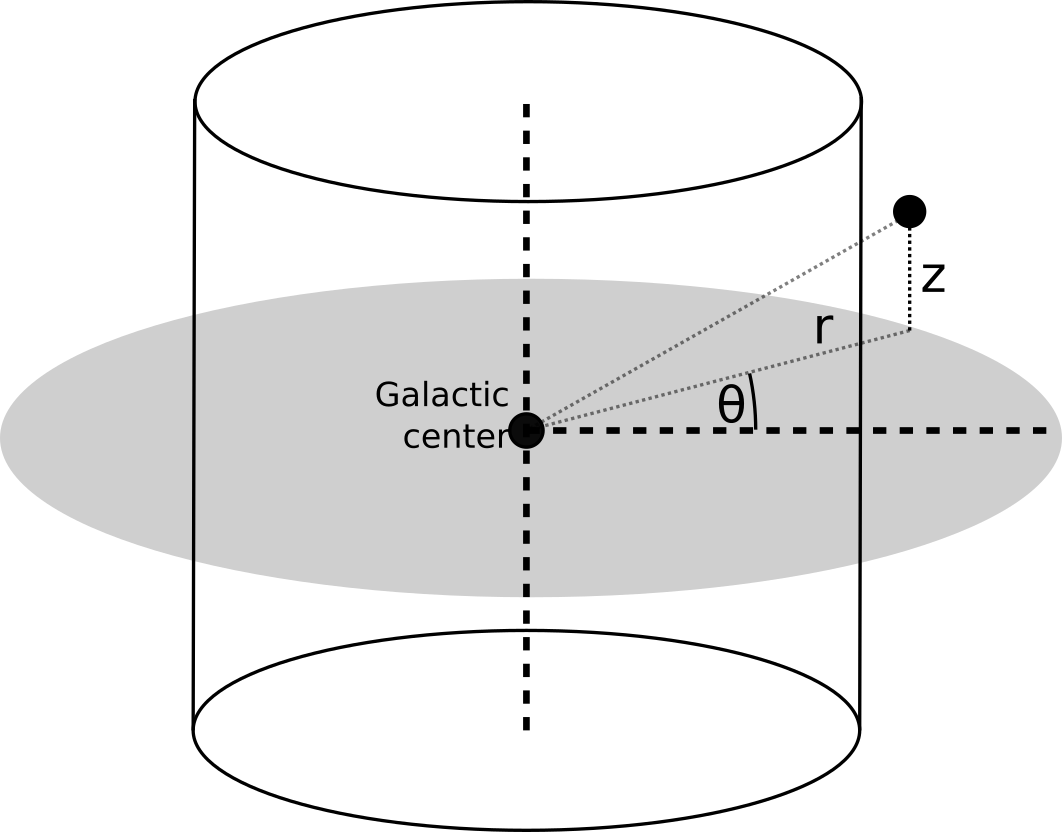
\includegraphics{imgs/cyl-coords}
    \caption{This figures shows the process of finding a cylindrical coordinate.}
    \label{cylindrical-coords}
\end{figure}

\subsection*{Local Standard of Rest}

Now that we have a definition of the cylindrical velocity coordinates, we can deine the Local Standard of Rest (LSR), an important concept in astrophysics. The LSR at a given moment is defined to be the velocity of a body in the sun's position, in a perfectly circular and on-plane orbit---which in practice means the $\Theta$-component of the sun's velocity, with $\Pi$ and $Z$ set to zero.

The velocity of a nearby star relative to the LSR is known as its \emph{peculiar velocity}, and approximates the velocity of that star relative to the sun. Its coordinates are typically designated $(u,v,w)$, where
\begin{align}
    u &= \Pi - \Pi_{LSR} \\
    v &= \Theta - \Theta_{LSR} \\
    w &= Z - Z_{LSR}
\end{align}

The average peculiar velocity for stars in the solar neighborhood is approximately zero, since the universe is mostly axisymmetric. However, individual peculiar velocities vary widely, with young main-sequence stars like the sun having low velocities and old, metal-poor red dwarfs having higher velocities. As discussed earlier, this is due to the additional orbital perturbations experienced by old stars, especially during the chaotic period of formation $\SI{9}{\giga\year}$ ago.





\chapter*{Conclusion}
         \addcontentsline{toc}{chapter}{Conclusion}
	\chaptermark{Conclusion}
	\markboth{Conclusion}{Conclusion}
	\setcounter{chapter}{4}
	\setcounter{section}{0}

\emph{The process by which the structure and dynamics of the MW were discovered was by no means trivial: Linblad [ref.] was a hero along with the other pioneers.  Buried in the galaxy they had some advantages compared to understanding, say, the Andromeda, but being in the disk causes huge difficulties, not the least of which is the dust.}

\section{More info}
And here's some other random info: the first paragraph after a chapter title or section head \emph{shouldn't be} indented, because indents are to tell the reader that you're starting a new paragraph. Since that's obvious after a chapter or section title, proper typesetting doesn't add an indent there.


%If you feel it necessary to include an appendix, it goes here.
    \appendix
      \chapter{The First Appendix}
      \chapter{The Second Appendix, for Fun}


%This is where endnotes are supposed to go, if you have them.
%I have no idea how endnotes work with LaTeX.

  \backmatter % backmatter makes the index and bibliography appear properly in the t.o.c...

% if you're using bibtex, the next line forces every entry in the bibtex file to be included
% in your bibliography, regardless of whether or not you've cited it in the thesis.
    \nocite{*}

% Rename my bibliography to be called "Works Cited" and not "References" or ``Bibliography''
% \renewcommand{\bibname}{Works Cited}

%    \bibliographystyle{bsts/mla-good} % there are a variety of styles available;
%  \bibliographystyle{plainnat}
% replace ``plainnat'' with the style of choice. You can refer to files in the bsts or APA
% subfolder, e.g.
 \bibliographystyle{APA/apa-good}  % or
 \bibliography{thesis}
 % Comment the above two lines and uncomment the next line to use biblatex-chicago.
 %\printbibliography[heading=bibintoc]

% Finally, an index would go here... but it is also optional.
\end{document}
